%! Author = itgramic
%! Date = 05.12.23

% Preamble
\begin{flushleft}
    \subsubsection{pg\_auto\_failover}
\end{flushleft}
\begin{flushleft}
    \paragraph{Core-Features}
\end{flushleft}
\begin{flushleft}
    \paragraph{Replikation}
\end{flushleft}
\begin{flushleft}
    \paragraph{Proxy}
    pg\_auto\_failover benötigt einen \Gls{HAProxy}, um Load Balancing usw. \cite{VYXTI7BS}
\end{flushleft}
\begin{flushleft}
    \paragraph{API / Skripte}

\end{flushleft}
\begin{flushleft}
    \paragraph{Architektur}
    Die Dokumentation von pg\_auto\_failover \cite{PZZIZ5RT} zeigt auf, wie der Failover funktioniert:
    \begin{figure}[H]
        \centering
        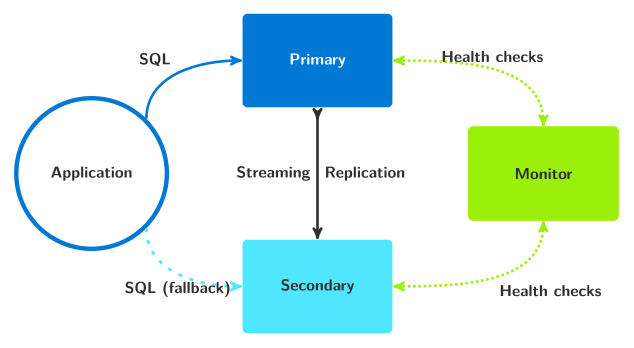
\includegraphics[width=0.75\linewidth]{source/implementation/evaluation/postgresql_ha_solutions/pg_auto_failover/pg_auto-failover_arch-single-standby}
        \caption{pg\_auto\_failover-Architektur - Single Standby}
        \label{fig:pg_auto-failover_arch-single-standby}
    \end{figure}

    Aber auch Multi-Nodes können eingebunden werden\cite{4ZKBDG57}:
    \begin{figure}[H]
        \centering
        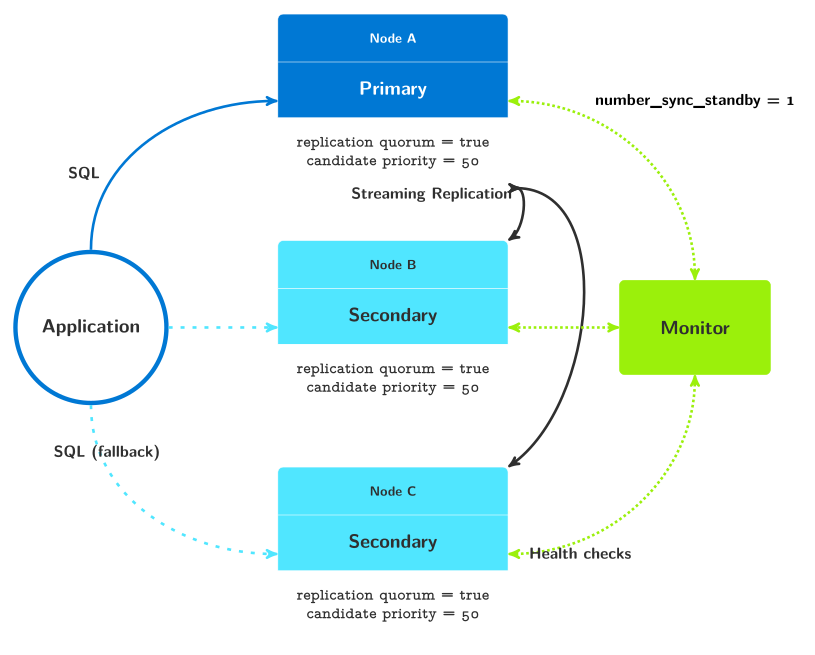
\includegraphics[width=0.75\linewidth]{source/implementation/evaluation/postgresql_ha_solutions/pg_auto_failover/pg_auto-failover_arch-multi-standby}
        \caption{pg\_auto\_failover-Architektur - Multi-Node Standby}
        \label{fig:pg_auto-failover_arch-multi-standby}
    \end{figure}

    pg\_auto\_failover kann Citus einbinden\cite{3FVHLIFE}.
    Allerdings bleibt die Architektur im Kern immer Monolothisch.
    \begin{figure}[H]
        \centering
        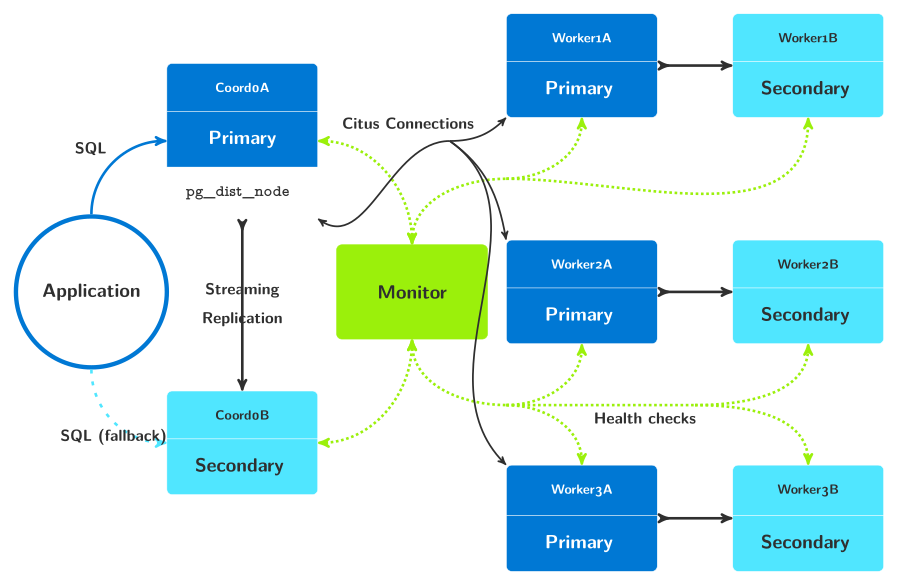
\includegraphics[width=0.75\linewidth]{source/implementation/evaluation/postgresql_ha_solutions/pg_auto_failover/pg_auto-failover_arch-citus}
        \caption{pg\_auto\_failover-Architektur - Citus}
        \label{fig:pg_auto-failover_arch-citus}
    \end{figure}
\end{flushleft}
\begin{flushleft}
    \paragraph{Synergien und Mehrwert}

\end{flushleft}